\documentclass{exam}
\usepackage[exos]{main}

\title{Propagations de rumeurs : meilleurs modèles}
\date{22 Avril 2024}
\author{Maths Spécifiques}

\begin{document}
\maketitle\thispagestyle{head}
\section{Rappels : Limites du premier modèle}
Nous sommes intéressés par un modèle de propagation des rumeurs. Ci-après, le modèle continu nous permet de considérer la quantité de personnes au courant d'une rumeur à n'\emph{importe quel instant $t$}. On note donc $f(t)$ le nombre de personnes au courant à l'instant $t$.
\begin{center}
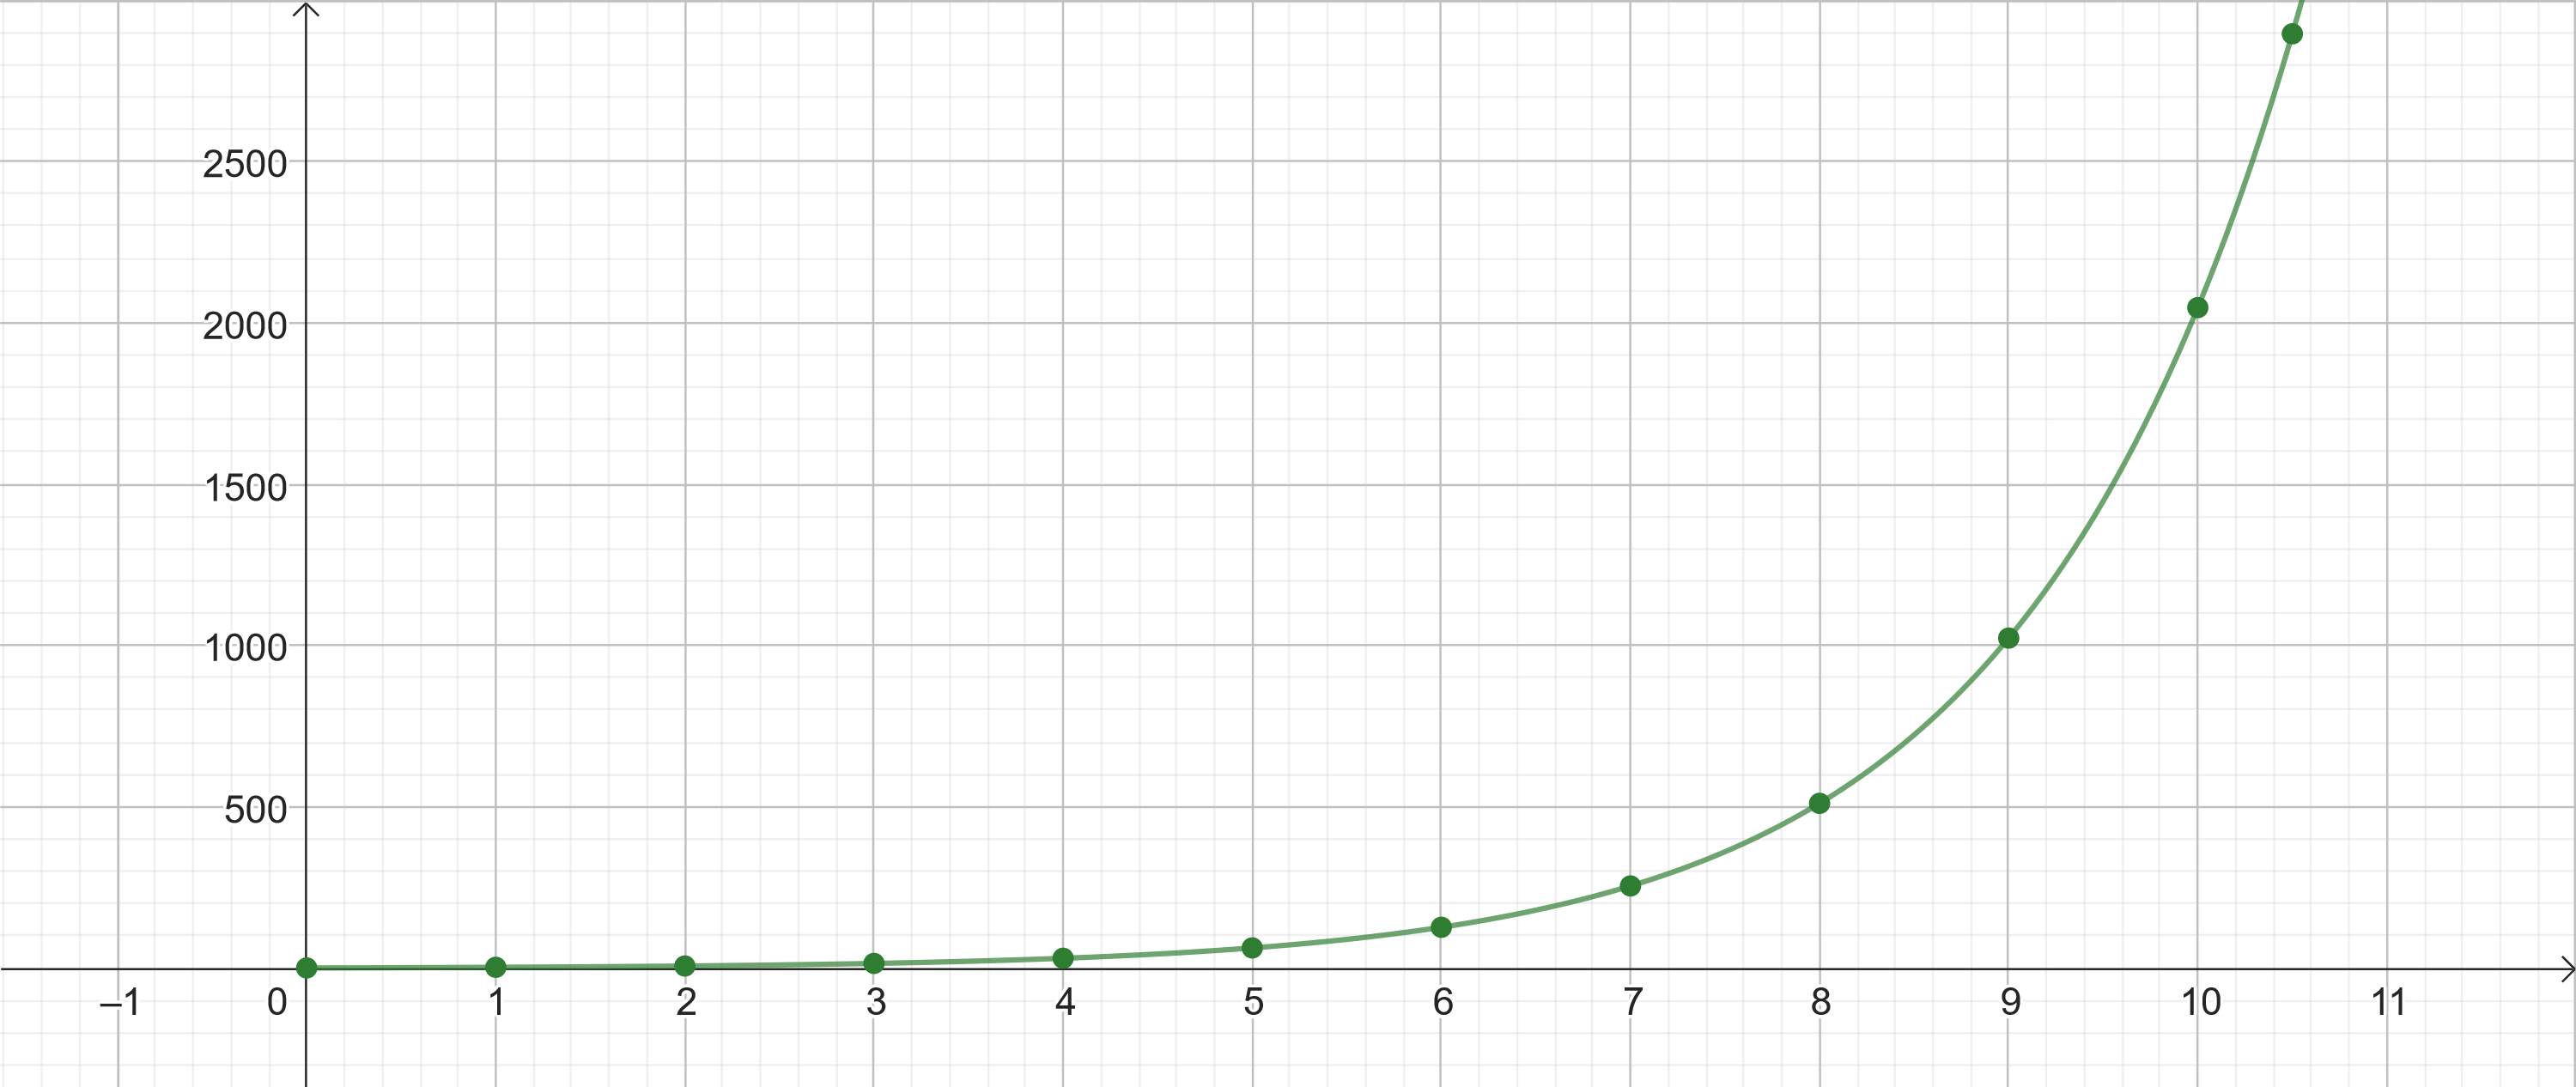
\includegraphics[width=0.9\textwidth]{Modele.png}
\end{center}
\begin{questions}
\question À partir de combien de temps $1500$ personnes sont au courant ? Cela vous paraît-il réaliste ?

\makeemptybox{4cm}
\question 
Pour quelle(s) autre(s) raison(s) ce modèle n'est-il pas réaliste selon vous ?

\makeemptybox{4cm}
\newpage
\section{Améliorations du modèle}
\question On se restreint à la propagation d'une rumeur dans un \emph{lycée de $1000$ personnes}. On propage une rumeur, et on mesure la quantité de personnes au courant toutes les dix minutes. Le résultat obtenu est donné par le graphique suivant.
\begin{center}
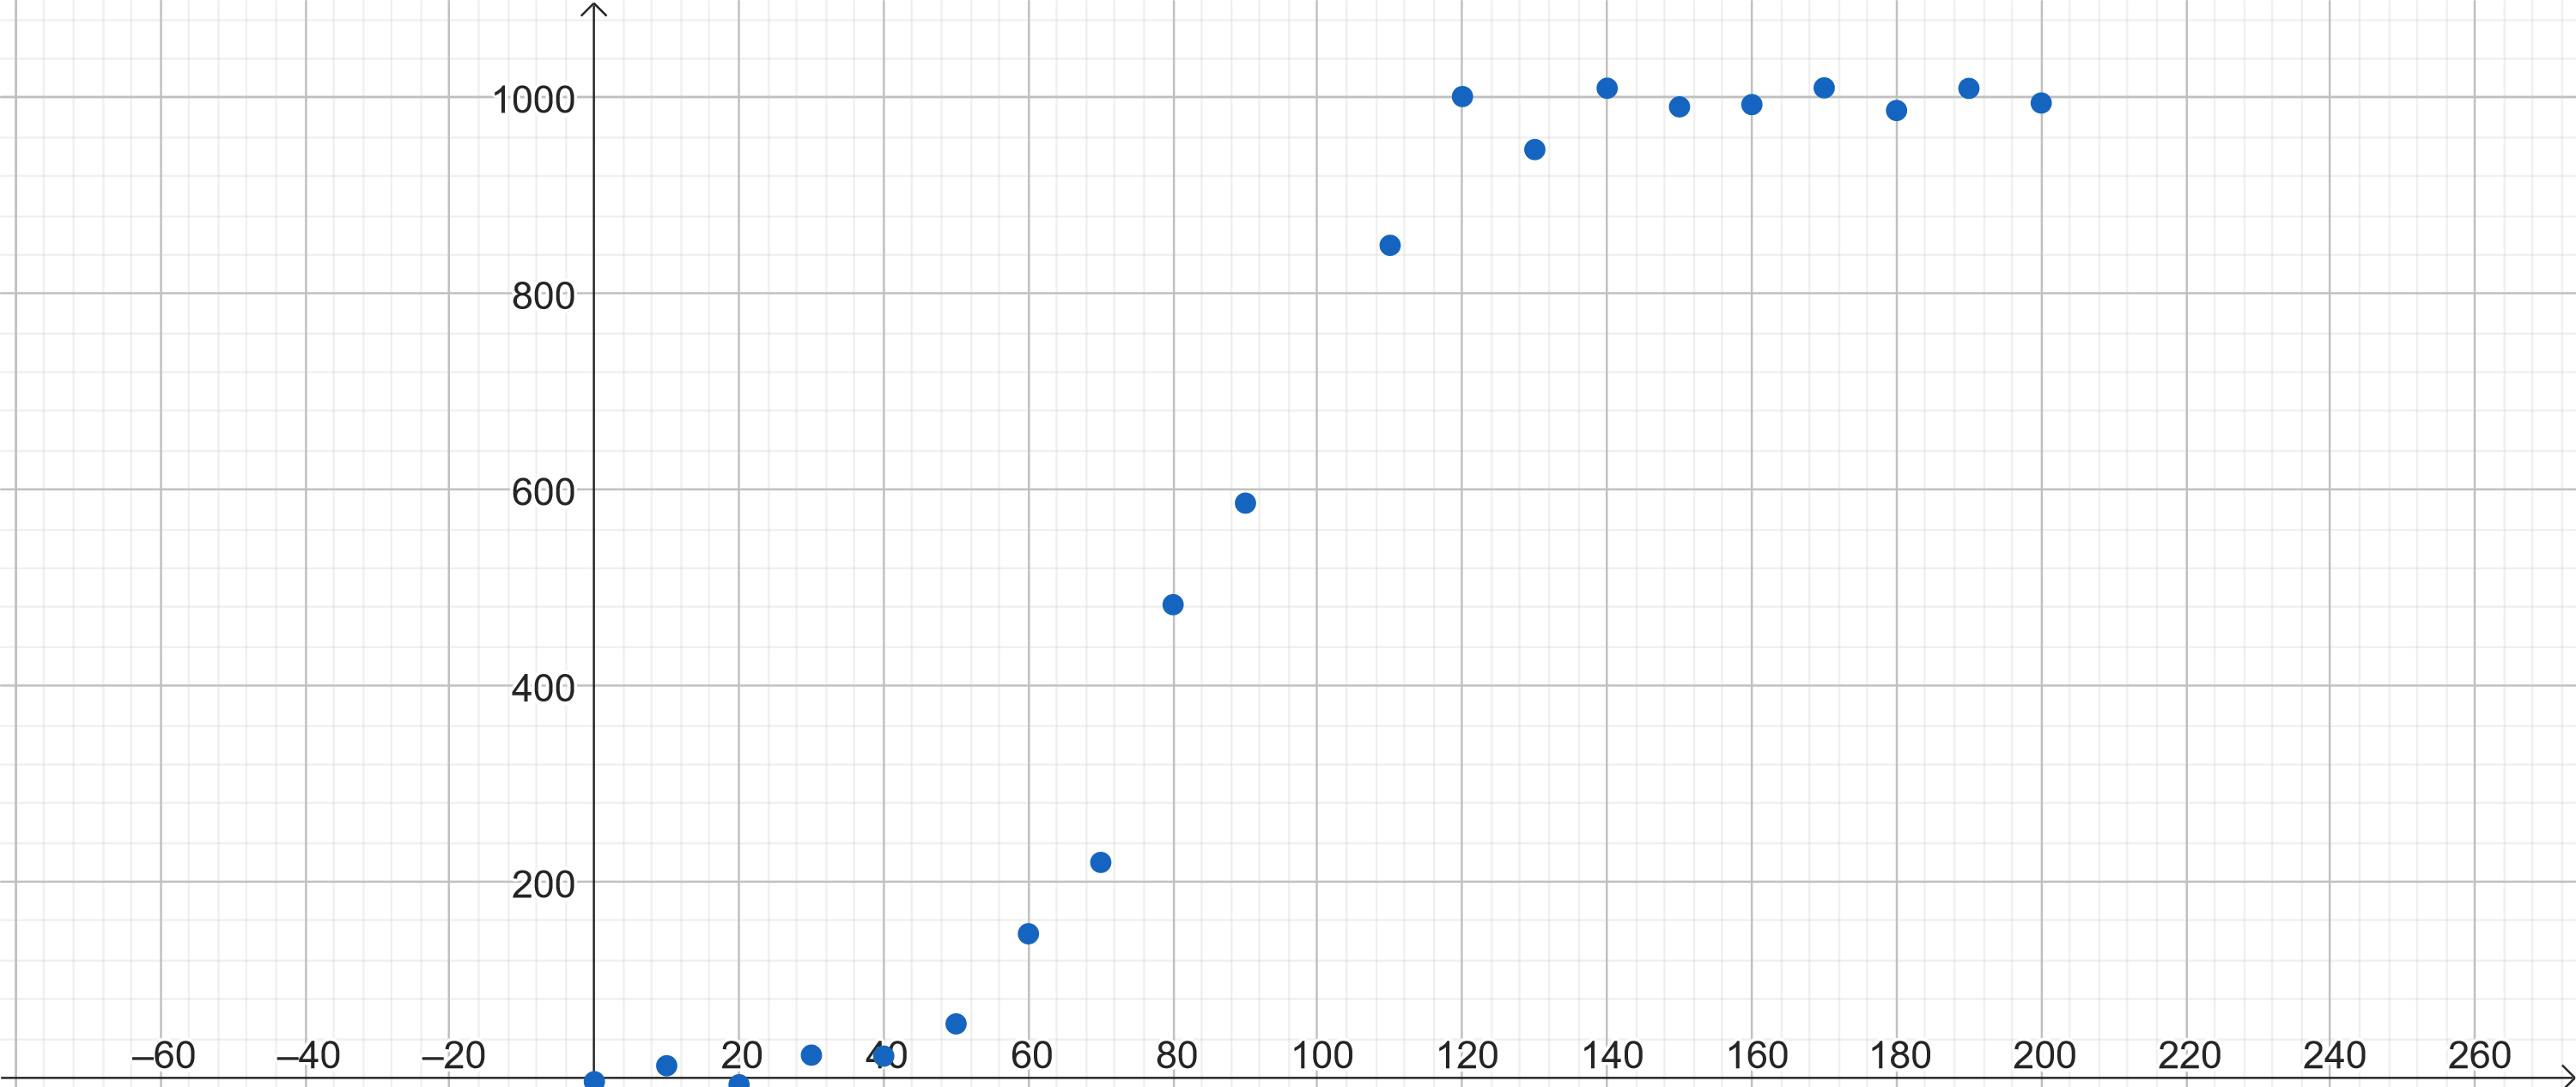
\includegraphics[width=0.9\textwidth]{Modele_sin.png}    
\end{center}
Pour quelle raison le graphique n'est pas vraisemblable ?

\makeemptybox{3cm}
\question On reproduit la même expérience, et on obtient le graphique suivant. On a aussi tracé la courbe représentative de $f : x \mapsto a^x$, pour un paramètre $a$ correspondant à l'expérience.
\begin{center}
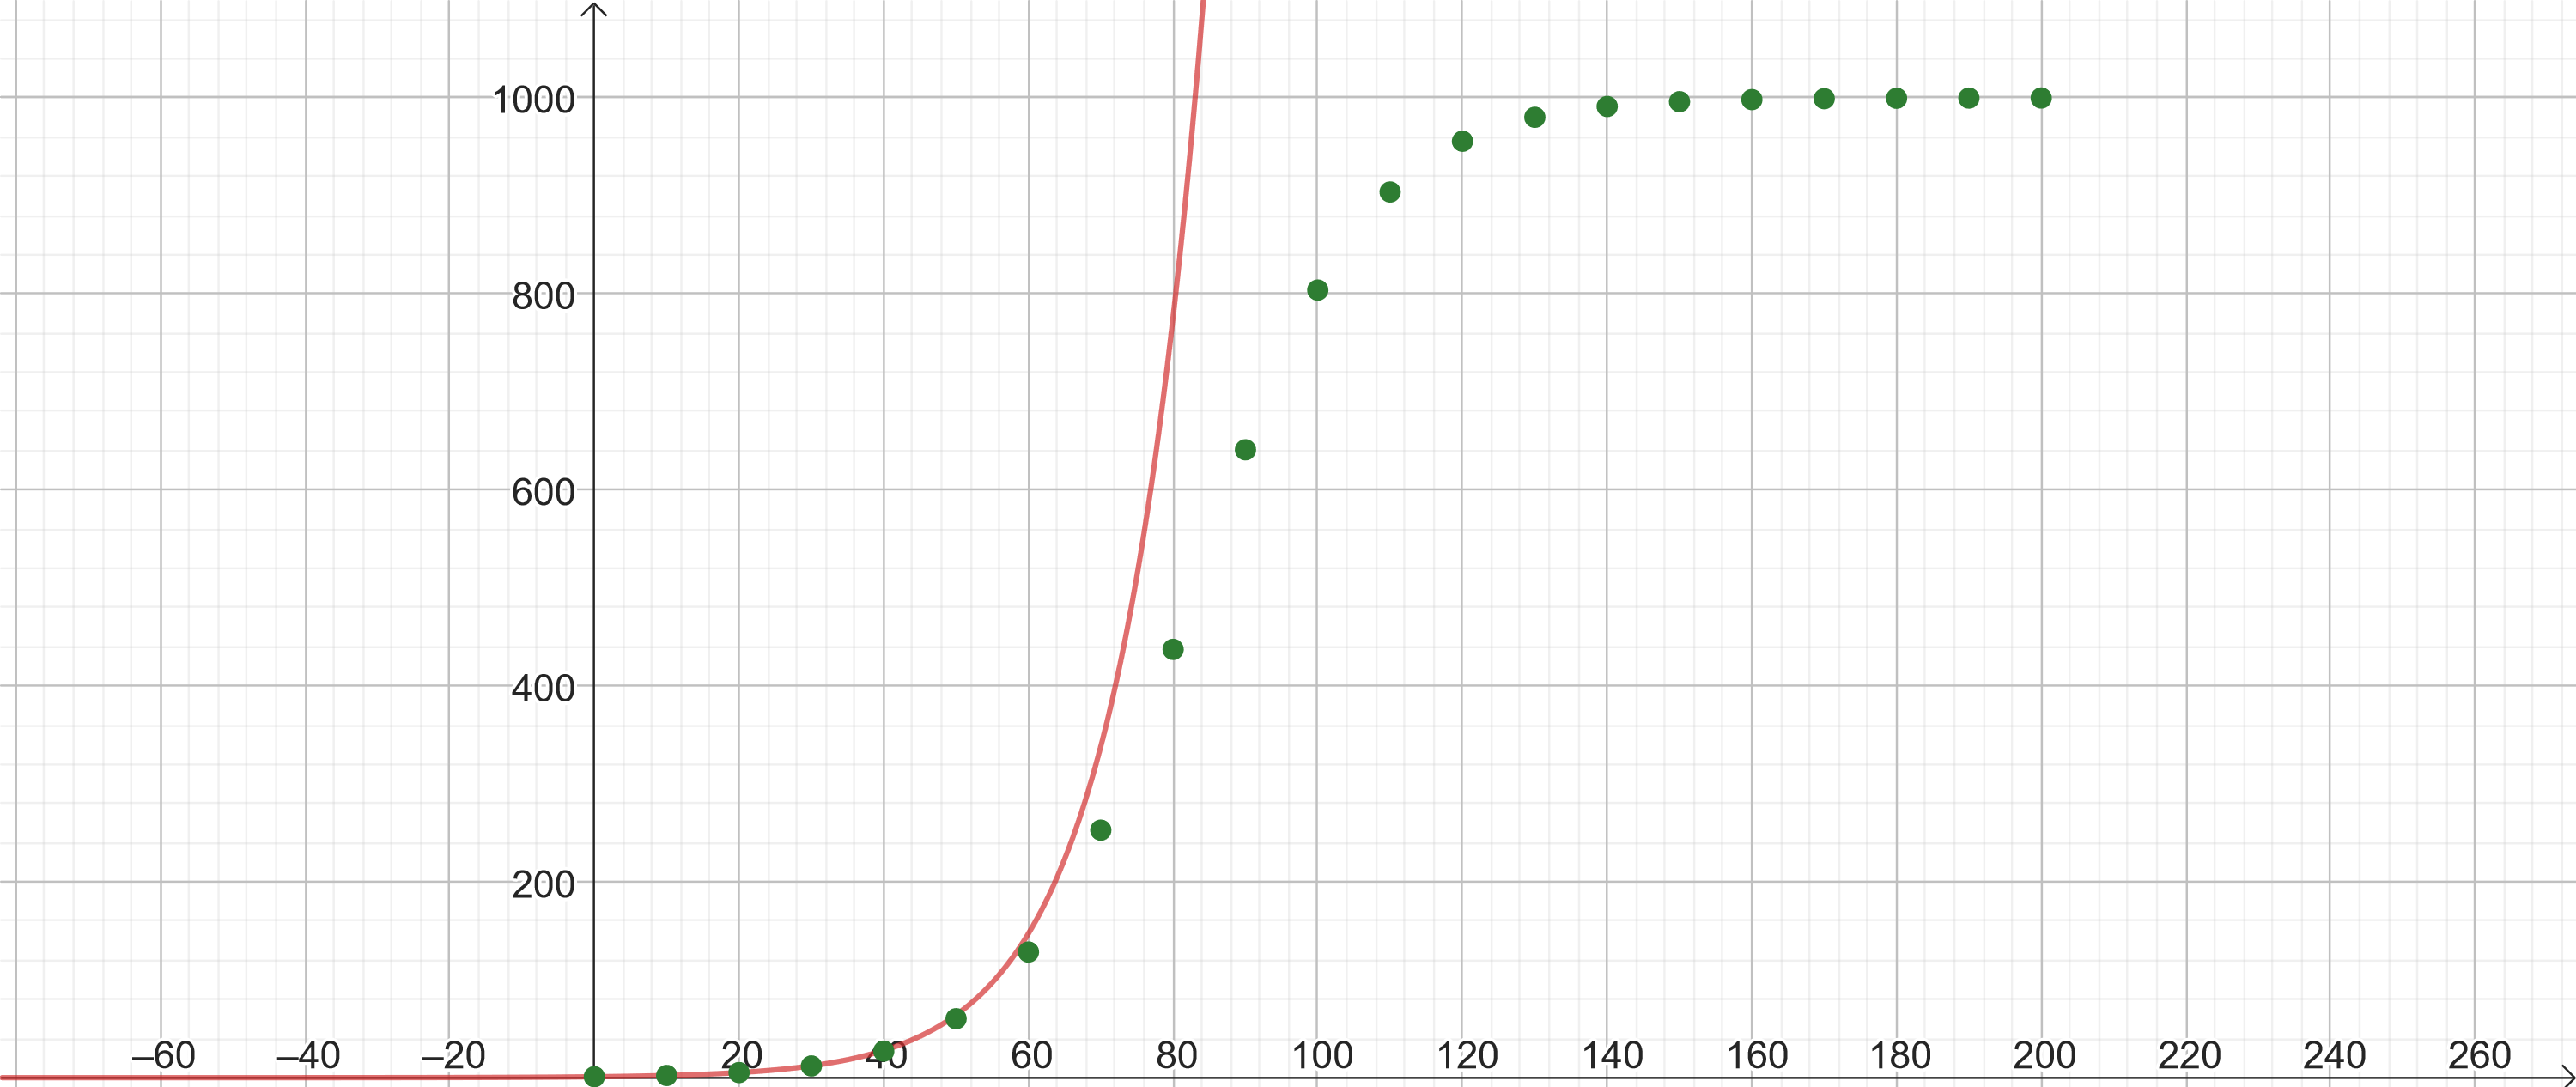
\includegraphics[width=0.9\textwidth]{modele_logistique.png}
\end{center}
\begin{parts}
\part Durant combien de temps la fonction $f$ est-elle adaptée pour modéliser la propagation de la rumeur ?
\makeemptybox{3cm}
\part Expliquer le comportement observé pour la propagation de la rumeur après deux heures.
\makeemptybox{3cm} 
\end{parts}
\section{Modèle Aléatoire}
\question Un autre modèle consiste à intégrer une dimension aléatoire à la propagation de la rumeur.
\begin{tcolorbox}
Au début de la propagation, une seule personne est au courant.
Chaque minute, toute personne au courant a une probabilité de $\dfrac{3}{4}$ de transmettre la rumeur à deux autres personnes.
\end{tcolorbox}
Les quatre graphiques suivants représentent quatre rumeurs différentes, et leur propagation sur $10$ minutes.
\begin{center}
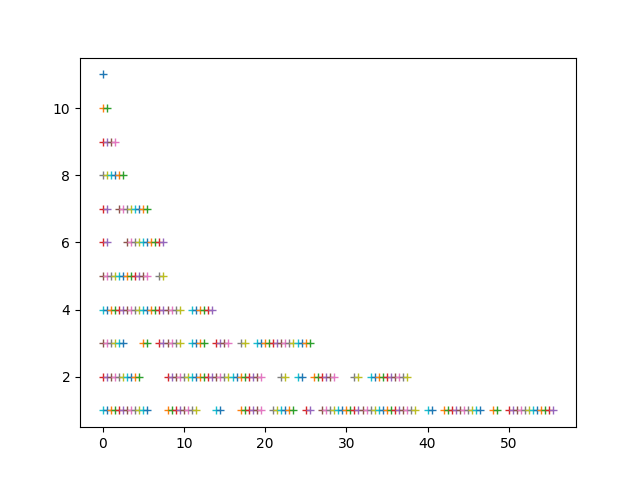
\includegraphics[width=0.45\textwidth]{ModeleAleatoire1.png}
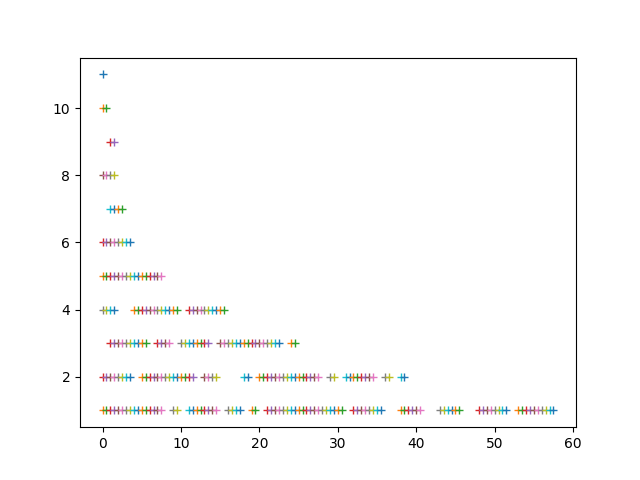
\includegraphics[width=0.45\textwidth]{ModeleAleatoire2.png}
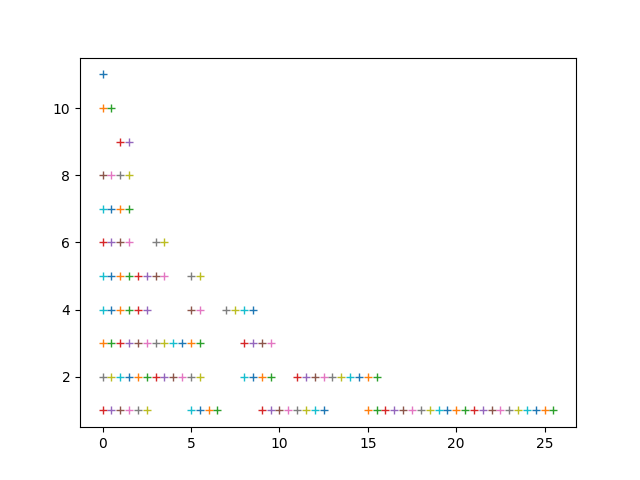
\includegraphics[width=0.45\textwidth]{ModeleAleatoire3.png}
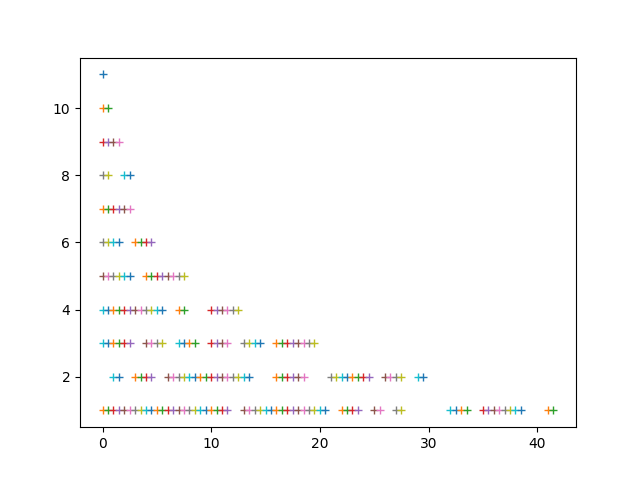
\includegraphics[width=0.45\textwidth]{ModeleAleatoire4.png}
\end{center}
Chaque symbole $+$ représente une personne venant d'apprendre la rumeur. La première ligne correspondant à l'instant $t=0$, quand la première personne vient d'apprendre la rumeur. 
\begin{parts}
\part Numéroter les quatre figures, et classer les quatre rumeurs de la moins répandue à la plus répandue. Justifier votre choix.
\makeemptybox{2cm}
\part Quelle est la probabilité qu'à l'instant $t=1$, $3$ personnes sont au courant de la rumeur ?
\makeemptybox{2cm}
\end{parts}
\end{questions}
\end{document}